
\section*{Problema P10.37}

\renewcommand*\thesection{10.37}
\numberwithin{equation}{section}

\begin{center}
    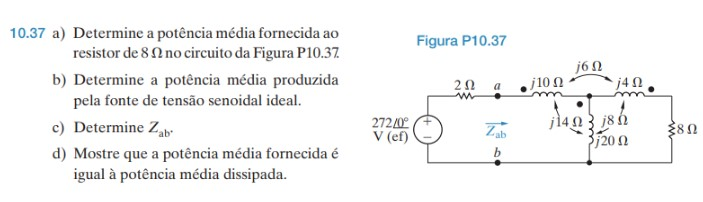
\includegraphics[scale=1.0]{P10.37.jpg}
\end{center}

\subsection*{(a)}

Aplicamos análise de malhas nas duas malhas do circuto, considerando as indutâncias mútuas. \\
Malha 1:

\[ - 272\phase{0^{\circ}} + 2I_1 + j10I_1 + j14I_1 + j14(I_1 - I_2) + j6(-I_2) + j8(-I_2) + j20(I_1 - I_2) = 0  \]

\[ I_1(2 + j10 + j14 + j14 + j20) + I_2(-j14 -j6 - j8 - j20) = 272\phase{0^{\circ}}  \]

\begin{equation}\label{eq:10.37.1}
    I_1(2 + j58) + I_2(-j48) = 272\phase{0^{\circ}}
\end{equation}

Malha 2:

\[ j20(I_2 - I_1) + j4(I_2) + 8(I_2) + j8(I_2) + j8(I_2 - I_1) + j6(-I_1) + j14(-I_1)  = 0 \]

\[ I_1(-j20 - j8 - j6 - j14) + I_2(j20 + j4 + 8 + j8 + j8)  = 0 \]

\begin{equation}\label{eq:10.37.2}
    I_1(-j48) + I_2(8 + j40) = 0
\end{equation}

Com \eqref{eq:10.37.1} e \eqref{eq:10.37.2}, temos o sistema linear

\begingroup
\renewcommand*{\arraystretch}{1.5}

\[
    \begin{bmatrix}
        2 + j58 & -j48    \\
        -j48    & 8 + j40
    \end{bmatrix}
    \begin{bmatrix}
        I_1 \\
        I_2
    \end{bmatrix}
    =
    \begin{bmatrix}
        272 \\
        0
    \end{bmatrix}
\]

\endgroup

Vamos resolver o sistema aplicando o método de Cramer. Temos

\begingroup
\renewcommand*{\arraystretch}{1.5}

\[ 
    \Delta
    =
    \begin{vmatrix}
        2 + j58 & -j48    \\
        -j48    & 8 + j40
    \end{vmatrix}
    =
    j544
\]

\[
    \Delta_{I_1}
    =
    \begin{vmatrix}
        272 & -j48    \\
        0    & 8 + j40
    \end{vmatrix}
    =
    2176 + j10880  \quad , \quad 
    \Delta_{I_2}
    =
    \begin{vmatrix}
        2 + j58 & 272    \\
        -j48    & 0
    \end{vmatrix}
    =
    j13056
\]

\endgroup

Assim, 

\[ I_1 = \frac{\Delta_{I_1}}{\Delta} = \frac{2176 + j10880}{j544} = 20 - j4 \un{A} \]

\[ I_2 = \frac{\Delta_{I_2}}{\Delta} = \frac{j13056}{j544} = 24 \un{A} \]

Calculadas as correntes de malha, temos a potência no resistor de $8 \;\Omega$ dada por

\[ \boxed{P_{8 \;\Omega} = R \cdot I_2^2 = (8)(24^2) = 4608 \un{W}}  \]

\subsection*{(b)}

A potência forncecida pela fonte é dada por

\[ S_{V_g} = V_g \cdot (I_1)^* = 272\phase{0^{\circ}} \cdot 20.39\phase{+11.31^{\circ}} = 5546.08\phase{11.31^{\circ}} \un{VA} \]

\[ \boxed{S_{V_g} = 5438.37 \un{W} + j1087.6 \un{VA}_R} \]

\subsection*{(c)}

Temos que $Z_{ab}$ é a impedância vista pela fonte, removido o resistor de $2 \;\Omega$. Logo,

\[ Z_{ab} = \frac{V_g}{I_1} - 2 = \frac{272\phase{0^{\circ}}}{20.39\phase{-11.31^{\circ}}} - 2 = 13.34\phase{11.31^{\circ}} - 2 \]

\[ \boxed{Z_{ab} = 11.08 + 2.62 \;\Omega} \]

\subsection*{(d)}

Vamos usar apenas a potência real (W). A potência real fornecida pela fonte é $P_{V_g} = 5438.37 \un{W}$. Os dois resistores
do circuito absorvem uma potência total de 

\[ P_{abs} = (2)|20 - j4|^2 + (8)(24)^2 = (2)(20.34)^2 + (8)(24)^2 = 5435.43 \un{W}  \]

Portanto, 

\[ \boxed{P_{abs} = 5435.43 \un{W} = P_{V_g}} \]









